\section{Results} \label{sec:results}
\subsection{Banner similarities}
\subsection{ISP}
\subsection{Reverse Geolocation}

With many major seaports, like Rotterdam, Antwerp and Hamburg, the North Sea has a lot of marine traffic. The sea also has a lot of offshore oil and gas fields; Ekofisk, Sleipner, Forties and Valhall, to mention a few.\cite{oil_field_lists} With this much activity within both constraints, the marine and offshore industries, a lot of things in the area have to be connected to the internet. To test if the IP geolocation services of Shodan could detect devices connected to the internet, a large area of the North sea was chosen: a circle with 270 km around 56\degree24\textquotesingle00.0N 3\degree00\textquotesingle36.0E, as seen in \cref{fig:geolocation}. To use Shodan to find devices within this area, the command \cref{lst:geolocation_sea} was used. As seen in the output from the command, no devices was found within the area.

\begin{figure} [H]
    \centering
    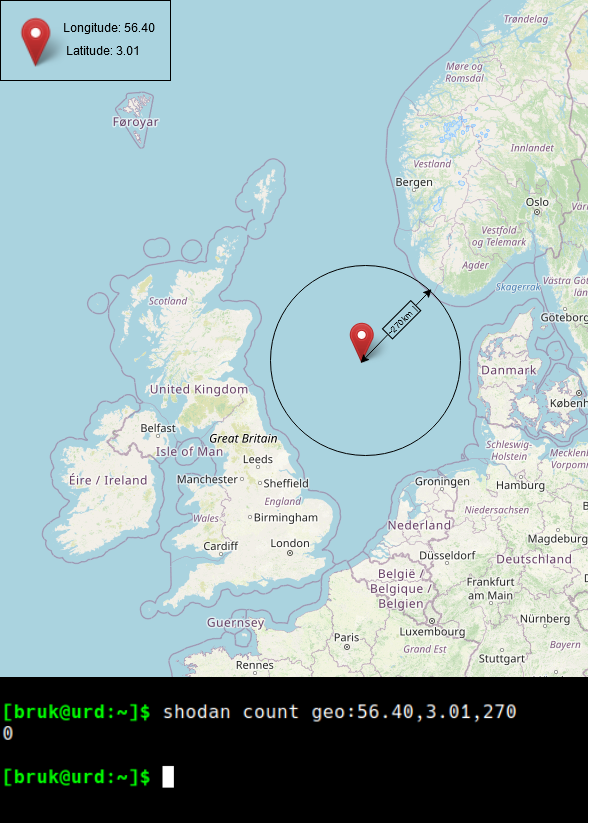
\includegraphics[scale=0.7]{Figurer/geolocation.png}
    \caption{Shodan "geo" filter visualized. Map copyright: https://www.openstreetmap.org/copyright}
    \label{fig:geolocation}
\end{figure}

\subsection{Latency and traceroute}
\subsection{Problems}
\subsubsection{NAT}
Due to NAT connecting devices to the internet trough a single router, Shodan will only scan the outer NAT routing device, and not the devices behind the NAT. NAT is not always used for getting more IPv4 addresses. Sometimes it is used purposely to hide IPv4 addresses from the public internet.

\subsubsection{firewalls}


